\documentclass{beamer}

\usepackage[utf8]{inputenc}
\usepackage[T1]{fontenc}
\usepackage{setspace}
\usepackage{color}
\usepackage{listings}
\usepackage{zi4}
\usepackage{tikz}
\usepackage{bchart}

\usetikzlibrary{positioning, arrows}

\usetheme{Frankfurt}

\lstset{basicstyle=\ttfamily,breaklines=true}

\definecolor{javared}{rgb}{0.6,0,0} % for strings
\definecolor{javagreen}{rgb}{0.25,0.5,0.35} % comments
\definecolor{javapurple}{rgb}{0.5,0,0.35} % keywords
\definecolor{javadocblue}{rgb}{0.25,0.35,0.75} % javadoc
 
\lstset{language=Java,
basicstyle=\footnotesize\ttfamily,
keywordstyle=\color{javapurple}\bfseries,
stringstyle=\color{javared},
commentstyle=\color{javagreen},
morecomment=[s][\color{javadocblue}]{/**}{*/},
%numbers=left,
%numberstyle=\tiny\color{black},
%stepnumber=1,
%numbersep=10pt,
tabsize=4,
showspaces=false,
showstringspaces=false}


\lstdefinelanguage{Bytecode}{
  keywords={GETSTATIC, INVOKEVIRTUAL, LDC, RETURN, ICONST, ALOAD, ASTORE},
  keywordstyle=\color{black}\bfseries,
  identifierstyle=\color{black},
  sensitive=false,
  comment=[l]{//},
  morecomment=[s]{/*}{*/},
  commentstyle=\color{purple}\ttfamily,
  stringstyle=\color{red}\ttfamily,
  morestring=[b]',
  morestring=[b]",
  basicstyle=\footnotesize\ttfamily
}

\begin{document}

\title[Optimization]
{Optimizing String manipulation performance}
\author{Markus Wondrak}
\institute
{
  Institute of Computer Science\\
  Johann Wolfgang von Goethe Universität, Frankfurt am Main
}

\frame{\titlepage}

\begin{frame}
  \frametitle{Table of Contents}
  \tableofcontents
\end{frame}

\section{Motivation}  

\frame{\sectionpage}

\begin{frame}[fragile]

  \frametitle{Example}
  \framesubtitle{The "normal" way}

  \begin{lstlisting}[language=Java]
String result = "";

for (int i = 0; i < line.length(); i += 2) {
  result += line.substring(i, i + 1);
}

return result;
  \end{lstlisting}%
\end{frame}


\begin{frame}[fragile]
  \frametitle{Example}
  \framesubtitle{The optimized way}
  \begin{lstlisting}[language=Java]
SubstringString lineOpt = new SubstringString(line);
  
StringListBuilder builder = new StringListBuilder();

for (int i = 0; i < line.length(); i+=2) {
  builder.append(lineOpt.substring(i, i + 1));
}

return builder.toString();
  \end{lstlisting}%
\end{frame}

\begin{frame}
  \frametitle{What is the difference?}
	\begin{itemize}
	  \item Java strings are immutable $\rightarrow$ manipulation causes \texttt{char[]} copy
	  \item '\texttt{+}' operator is compiled to a \texttt{StringBuilder}, {\bf but} the loop is not recognized
	  \item \texttt{StringBuilder} also array-based 

	  \item optimized types avoid this behavior 
	\end{itemize}
\end{frame}


\begin{frame}
  \frametitle{What is the difference?}
	\begin{itemize}
	  \item optimized types avoid this behavior 
	  \item \texttt{SubstringString} returns only a new object pointing to the new boundaries
	  \item \texttt{StringListBuilder} is a linked list
	\end{itemize} 
\end{frame}

\begin{frame}
  \frametitle{Measurement}

  \begin{bchart}[step=1000,max=3000]
    \bcbar[text=normal]{2956}
      \smallskip
    \bcbar[text=better*]{1138}
      \smallskip
    \bcbar[text=optimized]{1001}
    \bcxlabel{time in $ns$}
  \end{bchart}
  \\
  \vspace{1cm}
  \footnotesize (*) with the use of \texttt{StringBuilder} around the loop
\end{frame}

\begin{frame}
  \begin{center}
  \huge Wouldn't it be nice to have the performance of the optimized one with the readability of the normal one?
  \end{center}

\end{frame}

\begin{frame}
  \frametitle{Requirements}  
  Given a method optimization definition, the system should \dots
  
  \begin{itemize}
    \item \dots be applicable to to already compiled programs
    \item \dots identify method calls in the Java bytecode
    \item \dots replace these method calls by the optimized ones
  \end{itemize}
\end{frame}

\section{Bytecode}

\frame{\sectionpage}

\begin{frame}
   \frametitle{Bytecode}
   \begin{itemize}
      \item What the JVM actual executes (platform independence)
      \item Assembly language like 
      \item Stack-based and imperative
   \end{itemize}    
\end{frame}


\begin{frame}[fragile]
  \frametitle{Bytecode}
  Java:
  \begin{lstlisting}[language=Java]
String x = "Hallo Welt";
String y = x.substring(5);
  \end{lstlisting}%
  Bytecode:
  \begin{lstlisting}[language=Bytecode]
LDC "Hallo World!"
ASTORE 1
ALOAD 1
ICONST 5
INVOKEVIRTUAL java/lang/String.substring(I)Ljava/lang/String;
ASTORE 2
  \end{lstlisting}  
\end{frame}

\section{WALA}

\begin{frame}
  \frametitle{WALA}
  \begin{itemize}
    \item T.J. Watson Library of Analysis (IBM)
    \item static analysis for Java bytecode and Javascript
    \item open sourced at \texttt{http://github.com/wala/WALA} since 2006
  \end{itemize}

\end{frame}


\begin{frame}
  \frametitle{Features}
  
  \begin{itemize}
    \item Java type system and class hierarchy analysis
    \item supports frontends for Java and JavaScript
    \item SSA-based Intermediate Representation
    \item bytecode manipulation 
  \end{itemize}
  
\end{frame}

\begin{frame}
  \frametitle{Intermediate Representation}
  
  \begin{itemize}
    \item central data structure that represents the analyzed method
    \item abstracts the actual bytecode 
    \item is in static single assignment form
    \item consists of a control-flow graph 
    \item $\phi$-nodes represent a merge of variables 
  \end{itemize}     
   
\end{frame}

\begin{frame}[fragile]
  \begin{columns}
    \column{.45\textwidth}
    \begin{lstlisting}[language=Java]
String a = "test";
String b = "test2";		
String c = ((is) ? a:b);
		
return c.substring(9);
    \end{lstlisting}
    \column{.55\textwidth}
    \begin{figure}
      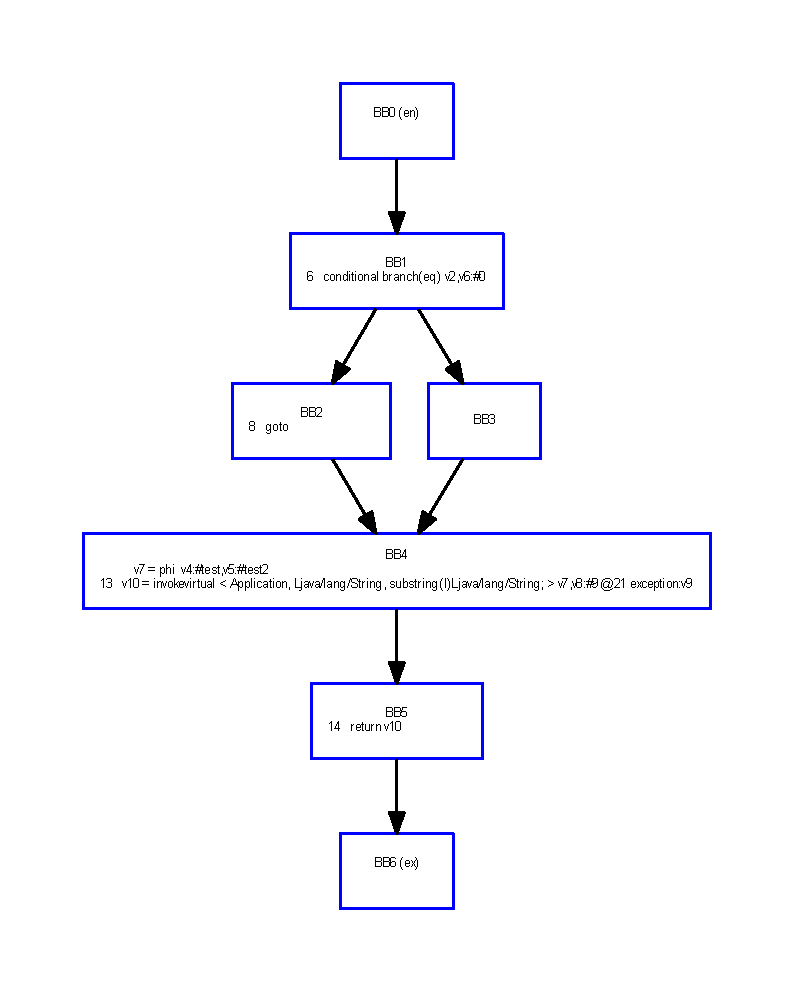
\includegraphics[scale=0.5]{irExample.pdf}
    \end{figure}
  \end{columns}
\end{frame}

\section{Analysis}

\frame{\sectionpage}

\begin{frame}
   \frametitle{Naming}
   \begin{block}{value number}
	   a variable in the IR
   \end{block}

	\begin{block}{local}
		a local variable in the bytecode
	\end{block}

	\begin{block}{label}
    a definition how certain method calls are identified and can be replaced
	\end{block}

\end{frame}

\begin{frame}
  \frametitle{Basic idea}
  \begin{itemize}
      \item Create a dataflow graph of the value numbers in the IR
      \item determine a bubble in that graph by
      \begin{itemize}
        \item label all affected method call instructions
        \item inherit the labels to all connected value numbers and instructions, if possible
      \end{itemize}
  \end{itemize}
\end{frame}

\begin{frame}
  \frametitle{How does the dataflow graph look like?}
  \begin{itemize}
    \item directed graph based on the IR
    \item is composed of 2 kinds of nodes
      \begin{itemize}
        \item \texttt{Reference} merely the value number ($R$)
        \item \texttt{InstructionNode} can be seen as a instruction  ($I$)
      \end{itemize}
    \item for $r\in R$, $i \in I$, 
    \begin{itemize}
      \item $(i,r)$ is called the definition of $r$     
      \item $(r,i)$ is called a use of $r$
    \end{itemize}
    \item $\forall r \in R, in(r) = 1$, so every $r$ has exactly 1 definition, but $n$ uses (SSA)
    \item $\forall i \in I, out(i) \leq 1$, so every $i$ can at most define one $r$
  \end{itemize}
\end{frame}

\begin{frame}
  \frametitle{InstructionNodes}
  
  \begin{itemize}
    \item \texttt{ConstantNode} a constant definition (e.g. \texttt{"Hallo World"})
    \item \texttt{ParameterNode} a parameter of the method
    \item \texttt{MethodCallNode} a method call (e.g. \texttt{x.f(y)})
    \item \texttt{ReturnNode} a return instruction of the method
    \item \texttt{PhiNode} a $\phi$ node in the IR
  \end{itemize}

\end{frame}


\begin{frame}
  \frametitle{example graph}
  \begin{center}

  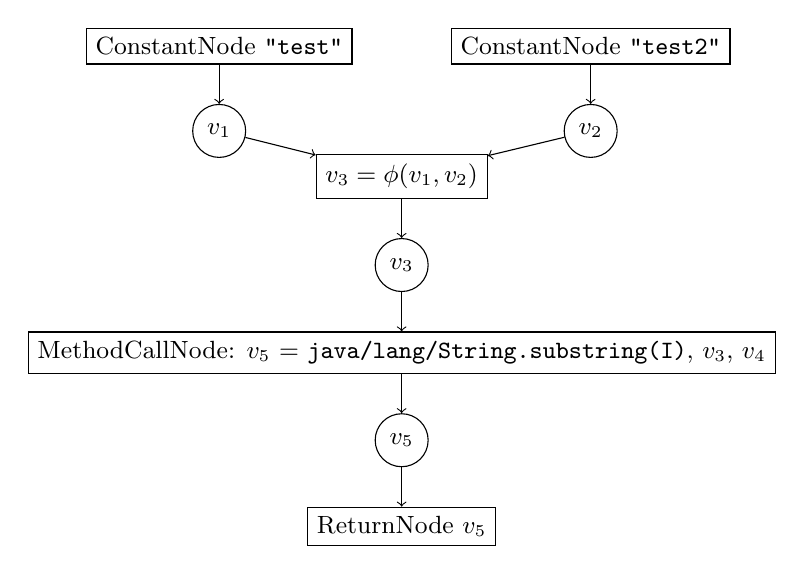
\begin{tikzpicture} [auto, node distance=0.5cm]
    \tikzstyle{every node}=[font=\small]
    \tikzset{
      inst/.style={draw=black, rectangle},
      ref/.style={draw=black, circle}
    }
    \node[inst]                       (constant1) {ConstantNode \texttt{"test"}};
    \node[right = of constant1]         (dummy1) {};
    \node[inst, right = of dummy1]       (constant2) {ConstantNode \texttt{"test2"}};
    
    \node[ref, below = of constant1]    (v1) {$v_1$};
    \node[below = of dummy1]            (dummy2) {};
    \node[ref, below = of constant2]    (v2) {$v_2$};

    \node[inst, below = of dummy2]       (phi) {$v_3 = \phi(v_1, v_2)$};
    \node[ref, below = of phi]          (v3) {$v_3$};    
    \node[inst, below = of v3]          (invoke) {MethodCallNode: $v_5$ = \texttt{java/lang/String.substring(I)}, $v_3$, $v_4$};
    \node[ref, below = of invoke] (v5) {$v_5$};    
    \node[inst, below = of v5] (return) {ReturnNode $v_5$};
    
    \draw[->] (constant1) to (v1);
    \draw[->] (constant2) to (v2);
    \draw[->] (v1) to (phi);
    \draw[->] (v2) to (phi);    
    \draw[->] (phi) to (v3);    
    \draw[->] (v3) to (invoke);    
    \draw[->] (invoke) to (v5);    
    \draw[->] (v5) to (return);    
    
  \end{tikzpicture}
  \end{center}
\end{frame}

\begin{frame}[fragile]
  \frametitle{How to define a label?}
  From the interface \texttt{TypeLabel}:
  \begin{lstlisting}
boolean canBeUsedAsParamFor(MethodReference,int)
boolean canBeUsedAsReceiverFor(MethodReference)
boolean canBeDefinedAsResultOf(MethodReference)
boolean canReturnedValueBeLabeled(MethodReference)
boolean compatibleWith(TypeLabel)
ReceiverInfo getReceiverUseInfo(MethodReference)
  \end{lstlisting}
\end{frame}

\begin{frame}
  \frametitle{How to deal with phis?}
  \begin{itemize}
    \item $\phi$-nodes just represent the merge of value numbers  
    \item any label could be compatible with any $\phi$ instruction
    \item so they where labeled after the analysis has taken place
    \item the decision is made by the count of labeled references connected to the particular phi
  \end{itemize}
\end{frame}

\section{Transformation}

\frame{\sectionpage}

\begin{frame}
	\frametitle{What to do?}
	\begin{itemize}
    \item Create conversation at the "bubbles" barriers
    \item replace the original method calls with the optimized ones
    \item to not overwrite the original values, create appropriate locals for the optimized ones
	\end{itemize}
\end{frame}

\begin{frame}
  \frametitle{local matrix}
  
  maxlocals are 6 and there are 2 labels ($l_1$,$l_2$):
  
  \begin{center}
    \begin{tabular}{c || c | c}
      original & $l_1$ & $l_2$ \\
      \hline 
      1 & 7 & 10 \\
      \hline
      2 & 8 & 11 \\
      \hline
      5 & 9 & 12 \\
    \end{tabular}
  \end{center}    
\end{frame}

\begin{frame}
	\frametitle{How to get the locals for a value number?}
	\begin{itemize}
    \item IR is an abstraction of the actual bytecode
    \item simple stack simulation tries to find the position at which the object is pushed onto / popped of the stack
 	  \item additionally save the position of the relevant (if any) \texttt{store} / \texttt{load} instruction 
    \item not possible for branches
	\end{itemize}
\end{frame}

\begin{frame}
  \frametitle{Conversations}  
  2 different scenarios:
  \begin{enumerate}
    \item \textit{The value is stored to a local}: Double the value and store it to the optimized local  
    \item \textit{The value is kept on the stack}: Convert the value on the stack
  \end{enumerate}
\end{frame}

\begin{frame}
  \frametitle{Method call replacement}  
  \begin{itemize}
    \item replace the load instruction to load the optimized type
    \item replace the method call itself to match the expected optimized type
    \item replace the store instruction to store the result to the optimized type
  \end{itemize}
\end{frame}

\section{Benchmarks}

\frame{\sectionpage}

\begin{frame}
  \frametitle{What are the results?}
  \begin{bchart}[step=2000,max=6000]
    \bcbar[text=normal]{2956}
      \smallskip
    \bcbar[text=optimized]{5583}
    \bcxlabel{time in $ns$}
  \end{bchart}
\end{frame}


\begin{frame}
	\frametitle{What went wrong?}

  \begin{itemize}
    \item Conversation are included into the measuring
  
  \end{itemize}

\end{frame}

\section{Conclusion}

\frame{\sectionpage}

\begin{frame}
	\frametitle{Conclusion}
	\begin{itemize}
    \item the system needs just the definition how to replace a certain method
		\item algorithm to determine the "bubble" is type independent, so not limited to \texttt{String}
		\item transformation on bytecode level makes the system applicable to already compiled programs (libraries in the classpath) 
	\end{itemize}
\end{frame}

\begin{frame}
	\frametitle{Future Work}
  \begin{itemize}
    \item loop sensitive \texttt{StringBuilder} optimization 
    \item inter procedural optimization would boost performance 
    \item a more offensive bubble growing strategy would cause a bigger bubble
    \item sources and slides at \texttt{github.com/wondee/faststring}
    \item because of Shrikes loose bytecode creation optimized classes need to be run with \texttt{-noverify}
  \end{itemize}
\end{frame}


\end{document}